\section{Methodology}
\begin{figure*}[htb]
    \centering
    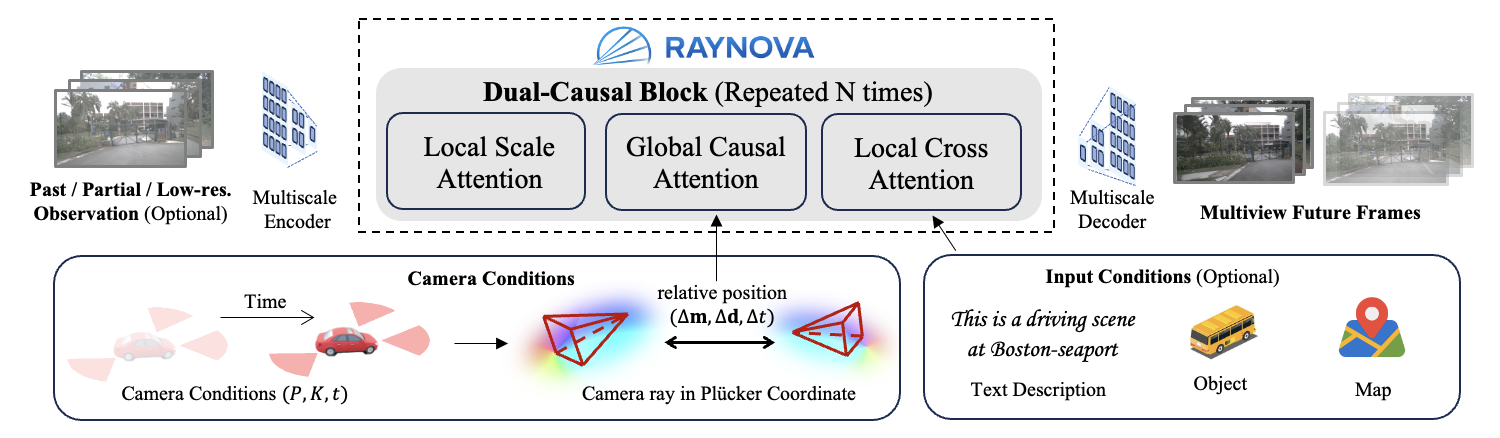
\includegraphics[width=\linewidth]{figs/overview.png}
    \vspace{-20pt}
    \caption{Overview of \ourmethod{} Framework. \ourmethod{} is composed of dual-casual (scale and time) blocks. The local scale attention and local cross attention works on each image indepedently, while the global causal attention works across multi-view and multiframe images enhanced with a unified ray-level relative position embedding for better spatio-temporal consistency.}
    \label{fig:overview}
\end{figure*}

\ourmethod{}, as shown in Fig.~\ref{fig:overview}, is a versatile world foundation model with autoregression. After introducing preliminary ``next-scale prediction" work (Sec.~\ref{sec:preliminary}), we formulate the dual-causal autoregressive framework for multi-view video generation in Sec.~\ref{sec:formulation}. Critical for coherent spatio-temporal reasoning, we construct an isotropic 4D position embedding based on the relative positions between camera rays in Sec.~\ref{sec:space}. This enables the development of a transformer-based geometry-free framework with minimal inductive biases for world modeling that takes diverse control signals in Sec.~\ref{sec:framework}. Finally, to alleviate the distribution drift in the autoregressive generation of long videos, we develop a recurrent training paradigm that aligns the distributions in the training and inference stages (Sec.~\ref{sec:training}).

\subsection{Preliminary: Next-Scale Prediction}
\label{sec:preliminary}
Unlike vanilla autoregressive models~\cite{lee2022autoregressive,yu2021vector} that flatten the 2D grids of images into 1D tokens, some recent work~\cite{tian2024visual,han2024infinity} shifts from ``next-token prediction” to ``next-scale prediction” strategy. Each image is quantized by the tokenizer into $K$ multiscale token maps $X_{1:K}=(X_1, X_2,\dots,X_K)$ with increasingly higher resolutions $h_k\times w_k, k=1,2,\dots,K$. The autoregressive likelihood is formulated as follows.
\vspace{-5pt}
\begin{equation}
    p(X_1,X_2,\dots,X_K)=\prod_{k=1}^Kp(X_k|X_1,X_2,\dots,X_{k-1})
    \label{eq:var}
\end{equation}
where $X_k$ is the token map at scale $k$ containing $h_k\times w_k$ visual tokens. The sequence $(X_1, \dots, X_{k-1})$ is the prefix context for the prediction of $X_k$. During the $k$-th autoregressive step, all $h_k\times w_k$ tokens are generated in parallel.


\begin{figure}[tb]
    \centering
    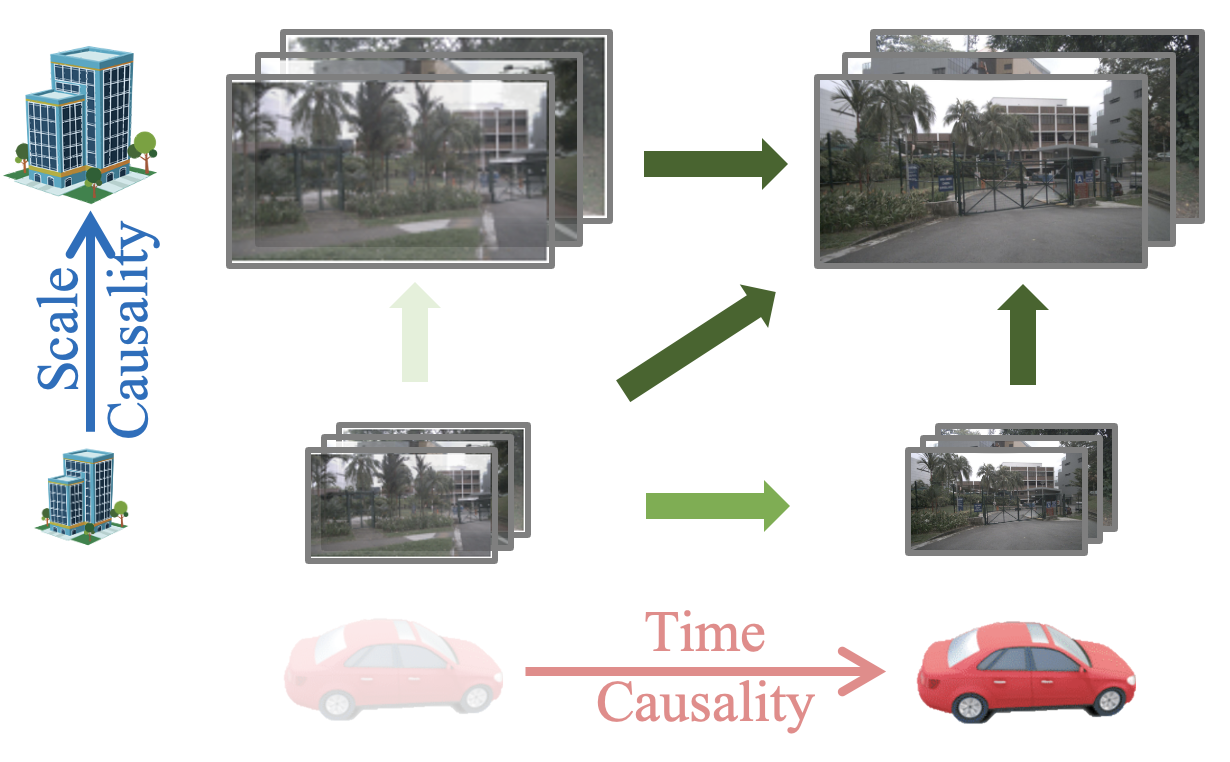
\includegraphics[width=0.9\linewidth]{figs/dual_causality.png}
    \vspace{-10pt}
    \caption{Dual-Causality for Multi-View Video Generation. \textcolor{darkgreen}{Green arrows} represent the causal dependency, while the darkness indicates the topological order of autoregression (from \textcolor{lightgreen}{light} to \textcolor{darkdarkgreen}{dark}).}
    \label{fig:dual-causal}
    \vspace{-5pt}
\end{figure}


\subsection{Formulation of Dual-Causal Autoregression}
\label{sec:formulation}
We formulate our proposed \ourmethod{} for world modeling via multi-view videos beyond image-level ``next-scale prediction". In favor of versatility, each image $I^{v,t}$ is tokenized independently as a multiscale token map $X^{v,t}_{1:K}$ for each frame $t=1,\dots,T$ and each camera view $v=1,\dots,V$. To model the joint distribution of multi-view and multi-frame images in a unified space, our autoregressive model considers two folds of causality: \textit{scale} and \textit{time} (Fig.~\ref{fig:dual-causal}). 

For the scale causality, we start from a single-frame case. The distribution of multi-view images in the same frame is modeled in a joint manner, since multi-view images describe a unified 3D space at a specific time step as a whole. For clarity, we omit the timestep superscripts.
\begin{equation}
p(X_1^{1:V},\dots,X_K^{1:V})=\prod_{k=1}^Kp(X_k^{1:V}|X_1^{1:V},\dots,X_{k-1}^{1:V}).
    \label{eq:scale}
\end{equation}

For time causality, the generation of each frame is conditioned on historical information. Different from some prior works~\cite{wen2024panacea,russell2025gaia2controllablemultiviewgenerative}, we do not assume strong inter-dependency among multi-frame images from the same camera since this inductive bias cannot be maintained with complex ego-motions (\eg turning). In contrast, we condition the multi-view image generation for the current timestep on all the views from past frames.
\vspace{-5pt}
\begin{equation}
p(X_{1:K}^{1:V,1:T})=\prod_{t=1}^Tp(X_{1:K}^{1:V,t}|X_{1:K}^{1:V,1:t-1}).
    \label{eq:time}
\end{equation}

Combining the scale and time causality from Eq.~\ref{eq:scale} and Eq.~\ref{eq:time}, we formulate the dual-causal block in \ourmethod{} as
\begin{equation}
p\left(X_{1:K}^{1:V,1:T}\right)=\prod_{t=1}^T\prod_{k=1}^Kp\left(X_{k}^{1:V,t}|X_{1:k-1}^{1:V,1:t}\right).
    \label{eq:formulation}
\end{equation}
It models the joint distribution of multi-view and multi-frame images with both spatial and temporal consistency.


\subsection{Isotropic Spatio-Temporal Representation}
\label{sec:space}

Inductive biases, such as multi-view adjacency or 3D latent features, in previous work limit their generalization in open world and adaptivity to heterogeneous data. Alternatively, we propose an isotropic 4D position embedding by extending the relative rotary position embedding~\cite{su2024roformer} to the camera ray space shared by all the multi-view and multi-frame visual tokens to enhance spatial and temporal consistency.

To this end, we start from a token-wise Pl\"ucker ray~\cite{plucker1865xvii} for the multi-scale feature maps. For convenience, we define a global 3D coordinate space whose origin is the ego-vehicle position at the first timestep. The extrinsic parameters for each camera view $v$ at each timestep $t$ are denoted as $\mathbf{P^{v,t}}$, while the intrinsic parameter is denoted as $\mathbf{K}^{v,t}$.\footnote{Although the intrinsic parameters are commonly fixed along the temporal dimension, we keep the superscript $t$ to tolerate special varying cases.} For each visual token $\mathbf{x}^{v,t}_k$ at scale $k$, it is straightforward to compute the corresponding Pl\"ucker ray $\mathbf{p}^{v,t}_k$ based on the camera parameters and its location in the image space. We further abuse this notation by appending an extra timestep $t$, so the extended Pl\"ucker ray is written as 
\begin{equation}
    \mathbf{p}^{v,t}_k=(\mathbf{m}_k^{v,t}\in\mathbb{R}^3,\mathbf{d}_k^{v,t}\in\mathbb{R}^3,t)
    \label{eq:ray}
\end{equation}
where $\mathbf{m}_k^{v,t}=\mathbf{o}^{v,t}\times\mathbf{d}_k^{v,t}$, camera center $\mathbf{o}^{v,t}$ is in the global coordinate system, and unit vector $\mathbf{d}_k^{v,t}$ is the ray direction.

Despite an intuitive approach that attaches the encoded Pl\"ucker ray to the corresponding visual token~\cite{jin2024lvsm,chen2024unimlvg}, this absolute position embedding has limited extrapolation ability beyond the scene range in the training stage, thereby hindering the model's generalization. To this end, we introduce \textit{relative embedding} that conditions networks on the relative position between camera rays using the modified self-attention blocks, where the attention score logit between two visual tokens is calculated as:
\begin{equation}
    a_{i,j}=\left(\mathbf{R}_{k_i}^{v_i,t_i}\mathbf{q}_{k_i}^{v_i,t_i}\right)^T\left(\mathbf{R}_{k_j}^{v_j,t_j}\mathbf{k}_{k_j}^{v_j,t_j}\right)={\mathbf{q}_{k_i}^{v_i,t_i}}^T\mathbf{R}_{\Delta}^{i,j}\mathbf{k}_{k_j}^{v_j,t_j}
    \label{eq:rope}
\end{equation}
where $\mathbf{R}_{\Delta}^{i,j}={\mathbf{R}_{k_i}^{v_i,t_i}}^T\mathbf{R}_{k_j}^{v_j,t_j}$ reflects the relative position between visual token $i$ and $j$ in the camera ray space. We derive $\mathbf{R}_{k}^{v,t}$ by extending RoPE to 7D space based on the Pl\"ucker ray (Eq.~\ref{eq:ray}). For clarity, we omit the superscripts and subscripts for scale $k$, camera view $v$, and timestep $t$. The rotary position encoding is written as:
\begin{equation}
    \mathbf{R}=\left[\begin{matrix}
        \mathbf{R_m} & 0 & 0\\
        0 & \mathbf{R_d} & 0\\
        0 & 0 & \text{RoPE}_{\frac{d}{4}}(t)
    \end{matrix}\right]\\
\end{equation}
where $\text{RoPE}_{\frac{d}{4}}(t)\in\mathbb{R}^{\frac{d}{4}\times\frac{d}{4}}$ is the 1D rotary position embedding~\cite{su2024roformer} for time step and $d$ is head dimension in the multi-head self-attention module~\cite{vaswani2017attention}. $\mathbf{R_m}$ and $\mathbf{R_d}$ refer to the rotary position encoding for $\mathbf{m}$ and $\mathbf{d}$ terms in the Pl\"ucker ray. Given their small scales, we multiply a scalar factor to each of them separately.
\begin{equation}
\begin{aligned}
    \mathbf{R_m}&=\left[\begin{matrix}
        \text{RoPE}_{\frac{d}{8}}(\mathbf{m}_1) & 0 & 0\\
        0 & \text{RoPE}_{\frac{d}{8}}(\mathbf{m}_2) & 0\\
        0 & 0 & \text{RoPE}_{\frac{d}{8}}(\mathbf{m}_3)\\
    \end{matrix}\right]\\
    \mathbf{R_d}&=\left[\begin{matrix}
        \text{RoPE}_{\frac{d}{8}}(\mathbf{d}_1) & 0 & 0\\
        0 & \text{RoPE}_{\frac{d}{8}}(\mathbf{d}_2) & 0\\
        0 & 0 & \text{RoPE}_{\frac{d}{8}}(\mathbf{d}_3)\\
    \end{matrix}\right]\\ 
\end{aligned}
\end{equation}

This relative position embedding considers visual tokens from all scales, views, and frames in a unified 4D space with minimal inductive biases, enabling generalization over long ranges and horizons. The model can adaptively learn interactions between visual tokens across spatial and temporal domains, and accommodate heterogeneous camera parameters and frame rates in training and inference.

\subsection{Dual-Causal Block Architecture Design}
\label{sec:framework}

We build a transformer-based framework for high-quality multi-view video generation upon a pretrained ``next-scale prediction" image generation model~\cite{han2024infinity} with minimal 3D inductive bias. In each transformer block, visual tokens are sequentially passed through an \textit{image-wise self-attention module} for image realism, a \textit{global self-attention module} for spatio-temporal consistency, and an \textit{image-wise cross-attention module} for conditional fidelity, as shown in Fig.~\ref{fig:overview}.

\paragraph{Image-wise self-attention for image realism.} The image-wise attention follows the design in  Infinity~\cite{han2024infinity}. Each image is processed independently, conditioned on its prefix scales, regardless of frames and camera views. Axial 2D RoPE~\cite{heo2024rotary} on the image space is adopted, which is normalized to a specific resolution for multi-scale features.

\paragraph{Global self-attention for spatio-temporal consistency.} Previous methods~\cite{wang2024driving,wen2024panacea,russell2025gaia} often apply separate spatial and temporal attention to reduce computational complexity. However, this decoupled design includes some prior assumptions about the camera motion and scene dynamics. In contrast, we propose a unified global attention based on the formulation in Eq.~\ref{eq:formulation} where each visual token attends to all its prefix in both scale-wise and temporal topological orders from all the camera views (Fig.~\ref{fig:dual-causal}). The relative position embedding explained in Sec.~\ref{sec:space} is also employed in this module to serve as a unified spatio-temporal representation. This module is implemented with masked self-attention during training, while the mask can be eliminated through proper KV-cache during inference. 
% Given the development in efficient attention kernels~\cite{dao2022flashattention,ansel2024pytorch}, this global module is not the bottleneck for either latency or memory compared to decoupled attention modules.

\paragraph{Image-wise condition alignment.} We apply an image-wise cross-attention module for input conditions, including text descriptions, 3D object bounding boxes, and HD maps. This module works on each image independently. The text descriptions are processed through a T5 encoder~\cite{raffel2020exploring}. For each object bounding box per frame, we project its eight corners to camera image space. It is possible that each box may be projected to one or more camera views. The projected coordinates of eight corners in the image space are encoded with MLP and then concatenated with the object category embedding from T5 encoder~\cite{raffel2020exploring} to obtain a high-dimensional latent feature. For the HD map, we sample several 3D points for each map element. In contrast to directly encoding the structural map element (\eg polylines or masks), this sampling approach is more flexible when dealing with unstructured or sketched maps. The points are projected to camera image space similar to object bounding box corners. The project coordinates of points belonging to the same map element are encoded with a lightweight PointNet-style network~\cite{qi2017pointnet}, and are then concatenated with the map element category embedding from the T5 encoder~\cite{raffel2020exploring} to obtain a high-dimensional feature. The latent features for text, object boxes, and HD maps are combined in the cross-attention module, allowing the visual tokens to attend to them simultaneously. For both objects and map conditions, we employ an Axial 2D RoPE~\cite{su2024roformer,heo2024rotary} between the features and tokens based on their projected centers in the image space. Experiments show that this relative position embedding can notably improve the locality of conditions.

Given the multi-view order-invariant nature of the above modules, we attach a frame-wise local absolute Pl\"ucker ray embedding in the beginning of our model to distinguish different views. The image-wise self-attention and cross-attention modules inherit the pretrained weights from Infinity~\cite{han2024infinity}, while the global self-attention module is randomly initialized and combined with zero-initialization~\cite{zhang2023adding}. This alternating local-global module can help balance the spatio-temporal consistency and per-image realism. 


\begin{algorithm}[tb!]
    \caption{\textbf{Recurrent Training for Long-Horizon Video Generation}}
    \label{alg:recurrent}
    \KwInput{Number of video frames $T$}
    \KwInput{Maximal cache length $M$}
    \KwInput{Multi-view video generation model that returns latent feature cache $G_{\theta}^L$}
    \KwInput{KV projection $\text{Proj}_{\theta}^{KV}$ (included in $G_{\theta})$}
    
    \Loop{
        Initialize KV latent feature cache $\mathbf{L}_{KV}\leftarrow[]$\\
        \For{$t\in1,\dots,T$}{
            $\mathbf{\tilde{x}}^t=\text{Random\_Bitwise\_Error}(\mathbf{x}^t)$\\
            \algcomment{Add random noise in scale-wise features to simulate the prediction errors}
            
            $\mathbf{KV}=\text{Proj}_{\theta}^{KV}(\mathbf{L}_{KV})$
            $\mathbf{\hat{x}}^t,\mathbf{l}_{KV}^t\leftarrow G_{\theta}^L(\mathbf{\tilde{x}}^t;\mathbf{KV})$\\
            \If{$\text{length}(\mathbf{L}_{KV})>M$}{
                $\mathbf{L}_{KV}\text{.pop}(0)$\\
            }
            $\mathbf{L}_{KV}\text{.append}\left(\text{stop\_grad}(\mathbf{l}_{KV}^t)\right)$\\
            \algcomment{Cache latents $\mathbf{L}_{KV}$ instead of $\mathbf{KV}$ to obtain gradient for $\text{Proj}_{\theta}^{KV}$ in past frames}

            $loss^t=\text{Cross\_Entropy}(\mathbf{\hat{x}}^t,\mathbf{x}^t)$\\
            Accumulate gradient of $loss^t$\\
            \algcomment{Per-frame backpropogation to save VRAM}
        }
        Update parameter $\theta$\\
        Clear accumulated gradient\\
    }
    % \algcomment{Generate the augmented copies for each sample} \\
    
\end{algorithm}


\subsection{Recurrent Training for Long-Horizon Videos}
\label{sec:training}

Given the GPU memory constraints, our autoregressive model training is limited to a few frames. Although it is extendable during inference through sliding windows, the generation of long-horizon videos suffers from distribution drift due to the gap between training and inference stages. 

To bridge this gap, we propose a novel training paradigm to align the training and inference distributions (Alg.~\ref{alg:recurrent}). It recurrently conducts forward and backward propagation frame by frame, and the gradients are accumulated until the end of each long sequence for model optimization. Obviously, the later frames are conditioned on the earlier frames. We cache the latent features in the global self-attention module since it is the only module operating across frames (Sec.~\ref{sec:framework}). While previous works often cache the keys and values separately~\cite{dai2019transformer,shoeybi2019megatron} during inference, we directly store the latent features before KV projection layer instead. In this case, we can 1) save half of the GPU memory and 2) ensure the KV projection layer in the computational graph, which is critical for temporal information extraction.

However, there is an error accumulation issue during inference since the ``next-scale prediction" framework takes ground-truth visual tokens as inputs during training. To this end, we draw inspiration from Infinity~\cite{han2024infinity} to randomly incorporate some mistakes in the visual token inputs during training to simulate the prediction errors during inference.
